% select subfiles base file
\documentclass[TGAI_Laborbericht.tex]{subfiles}
\begin{document}


\chapter{Versuch 2}
\label{chap:VERSUCH_2}


\section{Fragestellung, Messprinzip, Aufbau, Messmittel}
\label{chap:VERSUCH_2_FRAGESTELLUNG}
\subsection{Fragestellung}
In Versuch 2 erstellen wir nun die Spektren für die Wörter Hoch, Tief, Links, Rechts. Anschließend nehmen wir noch 5 Beispiele für diese 4 Wörter auf und vergleichen diese mit den Spektren. Anschließend nimmt ein anderer Sprecher nochmals je 5 mal die 4 Wörter auf und diese werden anschließend wieder mit dem Spektrum verglichen.

\subsection{Messprinzip}
Das Messprinzip ist das gleiche wie in Versuch 1.

\subsection{Aufbau}
Der Aufbau entspricht auch dem von Versuch 1.

\subsection{Messmittel}
Messmittel ist wieder das Mikrofon aus Versuch 1.

\section{Messwerte}
\label{chap:VERSUCH_2_MESSWERTE}
Um eine Referenz für jedes der Wörter Hoch, Runter, Links, Rechts zu erstellen nehmen wir jetzt jeweils 5 mal das jeweilige Wort mithilfe des Aufnahmeskriptes von Aufgabe 1 auf. Danach werden nochmals 5 mal das jeweilige Wort aufgenommen um zu verhindern, dass der Spracherkenner zu gut funktioniert. Anschließend nimmt ein anderer Sprecher auch nochmal 5 mal das jeweilige Wort auf.

\section{Auswertung}
\label{chap:VERSUCH_2_AUSWERTUNG}
Für jede der 5 Aufnahmen errechnen wir nun das Spektrum und ermitteln aus diesem dann den Mittelwert und erhalten so unsere Referenz. Nun schreiben wir uns noch eine Funktion um die Korrelation zu ermitteln. Hierzu nutzen wir die Funktion scipy.stats.pearsonr(). Nun vergleichen wir welches Spektrum die Höchste Korrelation mit der jeweiligen Aufnahme hat und können so ermitteln um welches Wort es sich handelt.

\begin{figure}[H]
	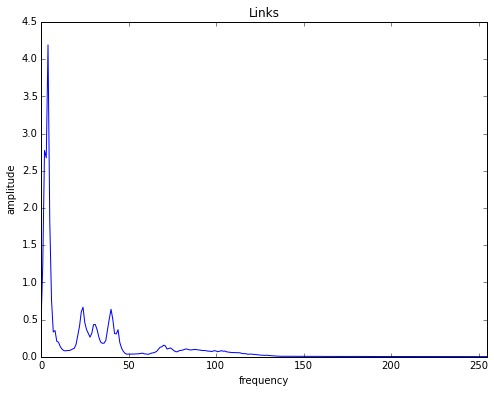
\includegraphics[width=0.7\textwidth]{media/links.png}
	\label{Links}
	\caption{Links}
\end{figure}

\begin{figure}[H]
	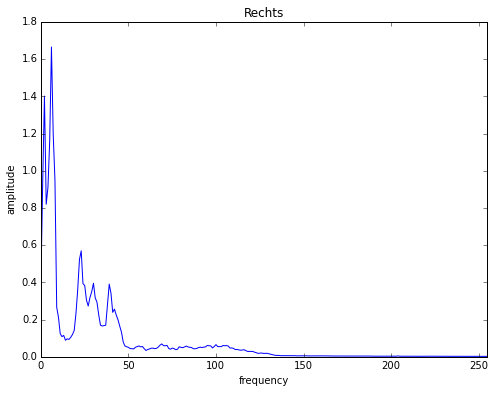
\includegraphics[width=0.7\textwidth]{media/rechts.png}
	\label{Rechts}
	\caption{Recht}
\end{figure}

\begin{figure}[H]
	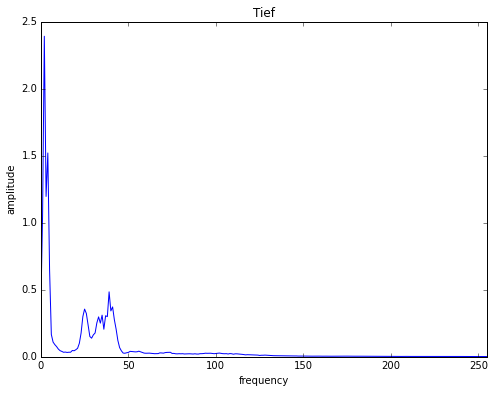
\includegraphics[width=0.7\textwidth]{media/tief.png}
	\label{Tief}
	\caption{Tief}
\end{figure}

\begin{figure}[H]
	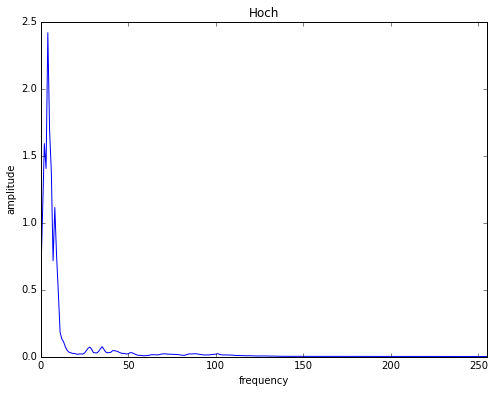
\includegraphics[width=0.7\textwidth]{media/hoch.png}
	\label{Hoch}
	\caption{Hoch}
\end{figure}


\section{Interpretation}
\label{chap:VERSUCH_2_INTERPRETATION}
Wir haben nun einen Funktionstüchtigen Spracherkenner. Mithilfe der Korrelation können wir nun die gesprochenen Wörter ermitteln.
So kommen wir auf eine übereinstimmung von 50\% bei dem Sprecher der die Referenz eingesprochen hat und auf 55\% beim anderen Sprecher.
Der Grund für die Ungenauigkeit könnte darin bestehen dass sich die Spektren der einzelnen Wörter, insbesondere Links und Rechts sehr ähneln.
\end{document}